The Web 2.0 revolution has given users of the internet many options to voice their opinion, for example social media platforms, product reviews or comments under blog posts and news articles.
This textual data can provide insights for researchers, analysts and policy makers. 
\begin{figure}[h]%
\label{screen}
\centering{%%
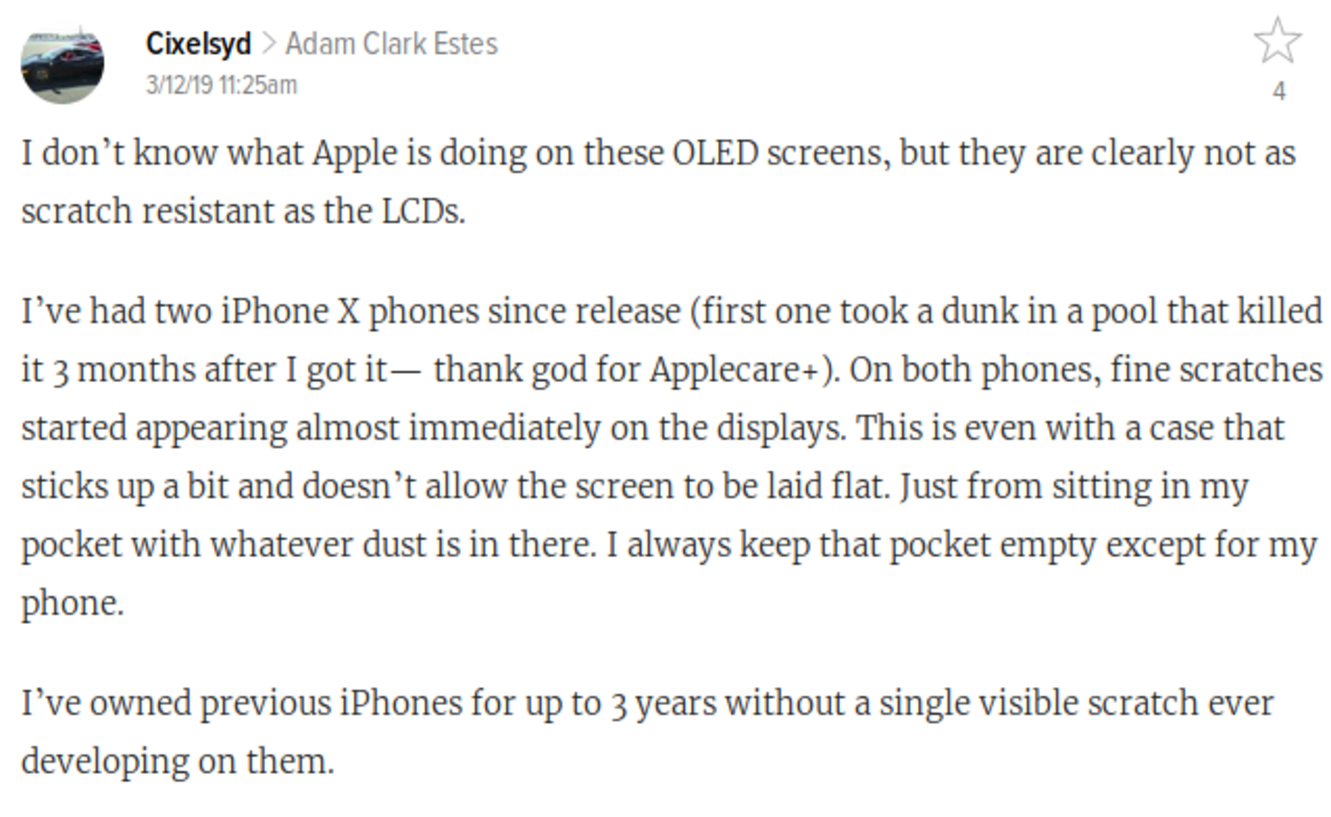
\includegraphics[width=0.45\linewidth]{img/screen1.pdf}}%
\qquad{%%
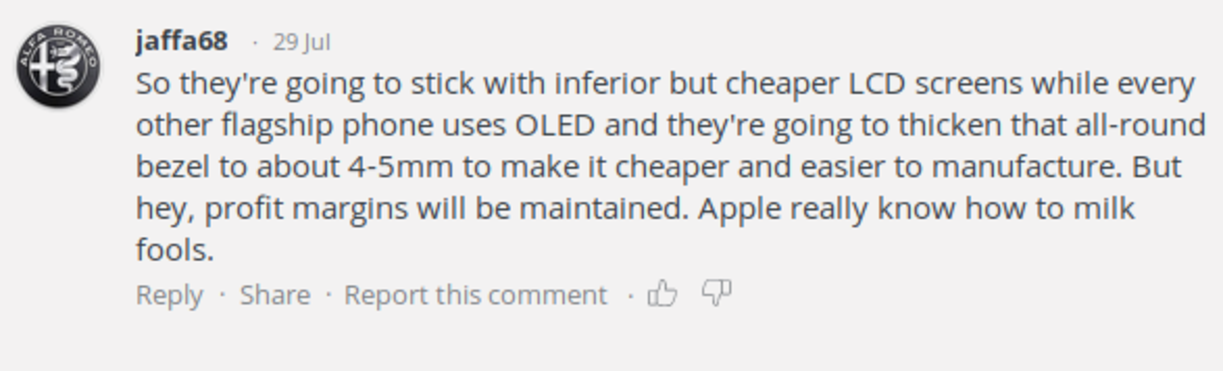
\includegraphics[width=0.45\linewidth]{img/screen2.pdf}}%
\caption{Two comments discussing a common topic under different articles.\protect\footnotemark}
\end{figure}
\footnotetext{Sources: \url{https://gizmodo.com/why-i-regret-upgrading-to-an-iphone-xs-1832653430}, \url{https://www.express.co.uk/life-style/science-technology/991936/iPhone-X-2018-release-best-look-yet-at-Apple-s-flagship-new-render-iPhone-X-Plus}}
\hyperref[screen]{Figure 1} shows two comments discussing different phone screen technologies under two different articles about iPhones\textsuperscript{\textregistered} (a registered trademark of Apple). While one talks favorably about OLED screens, the other prefers LCD screens as they seem more scratch-resistant. This is valuable information and depicts public opinion about a topic. However, the right comments are not always readily available.
The Huffington Post \footnote{\url{https://www.huffingtonpost.de/}}, for example, has reportedly received around 140,000 comments in a three-day period and news articles in the Guardian newspaper \footnote{\url{https://www.theguardian.com/international}} have gathered 25,000 to 40,000 comments a day \cite{DBLP:conf/ecir/AkerKBPBHG16} with single news articles receiving more than a thousand comments \cite{DBLP:conf/cikm/MaSYC12, llewellyn_grover_oberlander}.
Finding the relevant comments in such a large amount of data, which can also be meaningless and redundant, is exhausting, as Edmunds and Morris have pointed in a literature review on information overload in businesses \cite{Edmunds2000ThePO}. Nevertheless, filtering and summarization can provide relief \cite{Edmunds2000ThePO}. Many news outlets already offer filtering for news article comments. Particularly interesting comments are highlighted after editorial selection, for example \cite{DBLP:conf/icwsm/KhabiriCH11}, which is nevertheless inherently biased on the views of the editor \cite{DBLP:conf/icwsm/KhabiriCH11}. Intuitively, one might think that this can be alleviated when a sufficient number of, albeit non-professional, editors are involved through "Collaborative Recommendation" which is most frequently implemented in the form of up- and downvoting. This is contradicted by Chen et al. \cite{DBLP:conf/kdd/ChenGTY11} whose user study showed that there appears to be almost no correlation between rating and quality. Moreover, such mechanisms inherently suffer from an rich get richer effect \cite{DBLP:conf/cikm/MaSYC12}, which might omit important comments. Thus, there clearly is a need for more effective filtering techniques. \par
Text summarization as a field in Natural Language Processing (NLP) aims to reduce textual resources to the necessary bits under the preservation of the overall information content. It can ensure that an analyst of public opinion only sees necessary information but is not withheld important one.
This motivates the presented thesis to investigate the research problem of Text Summarization in the context of summarizing news article comments issued under multiple, topically related articles. Here, necessary bits of information are opinions on the topics discussed throughout the comments.
Topic modeling and graph clustering are used to find these topics and to group comments by their targeted topic, wherein the focus of the presented work lies. This work faces two challenges. First, the broad conversational structure under multiple articles with an unknown number of topics overlapping across comments and second, the data sparsity in usually short comment. The Hierarchical multi-Dirichlet Process (HMDP) topic model is introduced to improve topic modeling by accounting for the context under which comments are created, for example the date of its creation or its conversational thread.

\begin{figure}[H]
\label{figcontext}
	\centering
  \includegraphics[width=0.75\textwidth]{img/example_context.png}
	\caption{A comment thread snippet taken from an article about climate change of the Guardian newspaper \protect\footnotemark which illustrates the importance of context.}
\end{figure}
\footnotetext{\url{https://www.theguardian.com/commentisfree/2018/jul/09/the-guardian-view-on-climate-change-a-global-heatwave}}
The HMDP model is especially relevant for short comments, which are typically difficult to assign topics \cite{DBLP:conf/ecir/AkerKBPBHG16}. To employ an example, consider the comment thread from an article about global warming in \hyperref[figcontext]{Figure 2}. While the long comment can be clearly assigned a topic, the short ones cannot. However, with the contextual knowledge that both were issued under the article about global warming and as an answer to the comment above it can be assigned the topics of the comment it references. \par
The HMDP is compared to Latent Dirichlet Allocation (LDA) and the Markov Cluster Algorithm (MCL), which is graph-based and has found successful application in the clustering of comments of a single article. The comparison is based on a gold standard for which a creation process is outlined. Once comments are grouped by their topic, the most important negative and positive comments of the most important topic groups are extracted as a summary. Additionally, opinion is summarized in a visualization of sentiment. To establish importance, the ranking algorithm Maximal Marginal Relevance (MMR) is employed. Furthermore, topics are given a name through an introduced labeling algorithm. \par
To the best of the author's knowledge, this is the first work which explicitely aims to summarize comments under multiple news articles in a topic-driven manner. Related works either target single-article summarization \cite{DBLP:conf/cikm/MaSYC12, llewellyn_grover_oberlander, DBLP:conf/ecir/AkerKBPBHG16, DBLP:conf/ecir/FunkABPHG17} or present only comment snippets \cite{Raveendran:2012:LCS:2348283.2348490}.

\subsection{Problem statement}

\begin{definition}{Problem definition}
In this thesis, we focus on the extractive summarization of user comments under multiple, topically related news articles. The system shall be presented a set of articles $A=\{a_1,...,a_n\}$ and each of their associated comments $C_i = \{c_1,...,c_m\} \subseteq C$, where $C$ denotes all considered comments. It shall then output a summary of the main topics $T\prime \subseteq T$ in the form of an extracted subset of comments $C\prime \subseteq C$. Here, $T$ denotes the set of all topics discussed throughout the comments. The summary is required to not only present a reduced representation of the comments but also to preserve their overall meaning. \par
The focus of the presented work lies on the task of finding the topics discussed in comments and grouping comments by them. The main challenges which shall be adressed are mentioned in the following and considered in detail in later sections.
\begin{itemize}
\item An unknown number of topics.
\item Data sparsity of comments.
\item A broad conversational structure of comments under multiple related articles with overlapping topics, also across their comments, and a substantial temporal domain.
\end{itemize}
\end{definition}

\subsection{Thesis structure}
The rest of this thesis is structured as follows. Section 2 provides an overview over related works in Text Summarization and a technical background on topic modeling, clustering and fundamental text mining techniques. Readers who are already familiar with said techniques might skip parts of section 2.
Section 3 contains an overview of the chosen approach, a description of the data source and an analysis of characteristics of news article comments, on which the investigated topic modeling and clustering approaches are based. These are explained in section 4. This includes a description of how HMDP, LDA and MCL are used and how the topic labeling algorithm functions. Said methods are evaluated based on different criteria in section 5, followed by a discussion of the achieved results. The summary generation is outlined in section 6 with a description of ranking and selection and the chosen visualization.
In the end, a conclusion and possibilities for future work are presented.